\documentclass[10pt]{article}
\usepackage[T1]{fontenc}
\usepackage{lmodern,amsmath,amssymb,graphicx,hyperref}
\usepackage[margin=0.78in]{geometry}
\setlength{\parindent}{0pt}\setlength{\parskip}{6pt}
\begin{document}
\begin{center}
{\Large Actual first-jet factors with additive moment weights}\\[4pt]
43 authored statements, 14 November 2026\\
Source \texttt{6e97fcc1fffc1dcbdc25770aac701c2e252905c5}
\end{center}
\textbf{Result scope.} Constructed integral factors for the actual completed
first crossing jet, with $2^u k$ labels, normalized residual $k$, additive
weighted row profile $w+b$ and absolute residual $w+k$. These are unsigned
source-bound component claims [pcc:unverified].

\textbf{The same actual polynomial.} Keep the orientation-completed family
$W_{xy}(T)$, actual retained bit mask
\[
 M_{xy}=\{j<u:\operatorname{bit}_j(x)=\operatorname{bit}_j(y)\},
 \qquad \delta(x,y)=y-x.
\]
At $t=-2^i$, $i<u\le a$, let $J_{xy}$ be coefficient one of
$W_{xy}(t+2^{a+1}Z)$. The parent derives the actual nonzero diagonal
$c=J_{00}$ and $w=v_2(c)=a+1-i+G_i$. Let $R_{xy}=J_{xy}/c$ at equal-bit-$i$
crossings and zero elsewhere. All source ports are in $\mathrm{Fin}(2^a)$;
retained multiplicities are positive. Nodes, origin and source degree stay
those of this same completed family.

\textbf{Actual row coordinate.} Set
\[
 r=x\bmod2^u,\qquad h=x\mathbin{\mathrm{div}}2^u,
 \qquad x=r+2^u h.
\]
These are literal integer operations. The actual masks at $(x,y)$ and
$(r,y)$ agree. For the pole $q=t$ and each selected anchor $q=2^j$, define
\[
 d_q=q-\delta(r,y),\qquad e_q=2^u/d_q.
\]
Every relevant denominator is nonzero. Its actual valuation is at most
$i<u$ for the pole or $j<u$ for a selected anchor, hence $v_2(e_q)\ge1$.
The literal row identity gives
\[
 \frac{d_q}{q-\delta(x,y)}=(1+e_q h)^{-1}.
\]
No favorable denominator or scalar is supplied.

\textbf{Actual reciprocal family.} Polynomial derivative/first-jet
identities and exact finite products give
\[
 R_{xy}=R_{ry}/D_{ry}(h),\qquad
 D_{ry}(H)=(1+e_t H)\prod_{j\in M_{ry}}(1+e_j H)^{m_j}.
\]
The constructed finite polynomial depends on the retained row class $r,y$,
not its quotient $h$. Its constant is one. Convolution, finite products and
powers of the actual even slopes prove
\[
 \mathrm{VBound}(b,[H^b]D_{ry}),
 \quad \mathrm{VBound}(s,q)\equiv(q=0\lor v_2(q)\ge s).
\]
These are actual-family identities; no approximation oracle or desired
coefficient bound is assumed. PCC-20261114-84a6cb [pcc:unverified].

\newpage
\begin{center}{\Large Constructed inverse, truncation and finite error}\end{center}
For the actual weighted denominator $D$ with $D_0=1$, construct
$F=\operatorname{invOfUnit}(D,1)$ with the pinned standard power-series API.
Its explicit coefficient recurrence is
\[
 f_0=1,\qquad f_n=-\sum_{a+b=n,\ b<n}D_a f_b\quad(n>0).
\]
Strong induction proves $\mathrm{VBound}(n,f_n)$: every summand has additive
weight $a+b=n$, and finite sums preserve the bound. The actual constant-one
identity gives $DF=1$. This is a constructed inverse, not an assumed good
series. Standard inverse-series arithmetic is reused.

\textbf{Finite approximation.} For any $k\ge0$, define
\[
 Q_k(H)=\sum_{b<k}f_b H^b.
\]
Its coefficients retain their degree weights. The finite polynomial
$E=DQ_k-1$ has zero coefficients below $k$ by the exact formal inverse
identity; every coefficient $E_b$ retains valuation at least $b$. For any
actual integer $h$, each surviving term $E_bh^b$ has valuation at least $k$,
so
\[
 \mathrm{VBound}(k,E(h)).
\]
Only the finite polynomial $Q_k$ is evaluated. This error follows algebraically
from the finite residual $DQ_k-1$.

\textbf{Actual denominator unit.} The same weighted-coefficient argument
applied to $D-1$ gives $D(h)\equiv1\pmod2$. Consequently $D(h)\ne0$ and
$v_2(D(h))=0$. Dividing the finite residual derives
\[
 \mathrm{VBound}\bigl(k,D(h)^{-1}-Q_k(h)\bigr).
\]
All zero exclusions and unit valuation are derived. PCC-20261114-a88b83
[pcc:unverified].

Multiplying by the actual integral prototype $R_{ry}$ and using the exact
reciprocal-family identity gives
\[
 \mathrm{VBound}\bigl(k,R_{xy}-R_{ry}Q_k(h)\bigr).
\]
Prototype integrality comes from the parent's actual first-jet proof. The
row-class invariance of $D$ is established literally, so its coefficients
can be indexed by $r,y$ in the finite factors on the next page. Noncrossing
prototype entries are explicitly zero.

The proof retains the exact hypotheses on the original bit mask, finite
ports, positive multiplicities and retained level. It assumes neither the
desired matrix factorization nor a favorable truncation. Coefficient
construction and rational bit lengths still need complete cost accounting;
a valuation estimate alone does not price them.

\newpage
\begin{center}{\Large Explicit finite factors and actual weights}\end{center}
Labels are actual pairs $(r,b)\in\mathrm{Fin}(2^u)\times\mathrm{Fin}(k)$.
Writing $f_b(r,y)$ for the constructed inverse coefficient, define
\begin{align*}
 A_{x,(r,b)}&=[x\bmod2^u=r],2^b(x\mathbin{\mathrm{div}}2^u)^b,\\
 B_{(r,b),y}&=R_{ry}\,f_b(r,y)/2^b.
\end{align*}
If $r,y$ is noncrossing then $B=0$. Otherwise the actual prototype is
integral, and the derived coefficient weight $b$ cancels the exact
valuation of $2^b$. Thus
\[
 \mathrm{VBound}(b,A_{x,(r,b)}),\qquad
 \mathrm{VBound}(0,B_{(r,b),y}).
\]
No favorable integral factor is supplied. PCC-20261114-3be17e [pcc:unverified].

\textbf{Exact product.} The class selector leaves one literal residue
$r=x\bmod2^u$. The factors $2^b$ cancel, and the finite sum over $b<k$ is
exactly the constructed polynomial evaluation. Therefore
\[
 (AB)_{xy}=R_{ry}Q_k(h),\qquad
 \mathrm{VBound}(k,R_{xy}-(AB)_{xy}).
\]
All crossings and noncrossing zeros are included. PCC-20261114-15d101
[pcc:unverified].

\textbf{Absolute weights.} Multiply the actual row factor by the derived
$c$. The exact matrix-product scaling gives
\[
 \mathrm{VBound}(w+b,(cA)_{x,(r,b)}),\qquad
 \mathrm{VBound}(w+k,(J_{\rm cross}-cAB)_{xy}).
\]
Feasibility $G_i\ge0$ makes $cA$ integral as well. The weights are additive:
$w+b$, without a product of the gain and moment degree.
PCC-20261114-e3550d/f04bf6 [pcc:unverified].

\textbf{Charged count.} The exact number of inner labels is
\[
 \#\bigl(\mathrm{Fin}(2^u)\times\mathrm{Fin}(k)\bigr)=2^u k.
\]
For $k=0$ the factors are empty and the residual bound is zero bits. For
$k\ge1$, $k\le2^{k-1}$ gives
\[
 2^u k\le2^{u+k-1},
\]
the earlier row-refinement upper count when $u+k-1\le a$. This comparison
is between symbolic label counts. It is not a timing or complete bit-cost
comparison with the prior source's existing linear-moment method. At $k=1$
it matches the independently proved necessary count $2^u$ for this actual
first-jet precision. PCC-20261114-f6a09d [pcc:unverified].

Every retained mask is charged. The factor $2^u$ can exceed the old
$2^{i+1}$ tile count. All required higher chart jets and the full source
mode/precision/recovery/entry/recursion interface remain separate obligations.

\newpage
\begin{center}{\Large Evidence and remaining algorithmic obligations}\end{center}
\begin{center}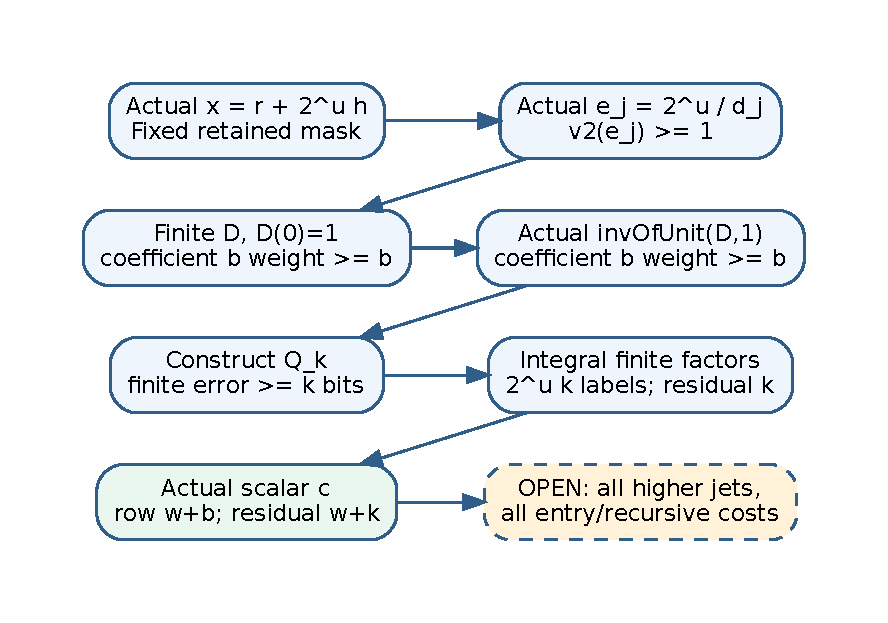
\includegraphics[width=0.88\textwidth,height=0.43\textheight,keepaspectratio]{research/prime_orientation_layers_20261114/moments/report/moments.pdf}\end{center}

\textbf{Formal artifacts.} One module contains43 authored statements.
Pinned shared gate audits44 declarations, including generated
\texttt{momentRight.congr\_simp}, with0 extra trusted axioms, exit0.
Import-inclusive fresh OrientationMoment is running at this checkpoint.
All exact source-bound records are unsigned; gate data PCC-20261114-24441c
[pcc:unverified].

\textbf{Separate higher-chart draft.} Seven isolated statements locally
derive actual retained crossing base content $a+1-i$, whole completed crossing
chart content $w$ and coefficientwise integrality after division by the actual
$c$. They are outside this43/44 audit/fresh, unsigned data310194. They provide
no higher-chart factorization [pcc:unverified].

\textbf{Evidence preservation.} Source/dependency pins, all failed drafts
and exact raw logs are retained. No old source, claim body or canonical ledger
history is rewritten. Parent fixed literal scaling certificate checks its
stated ring rearrangement only; no new native crypto fixture, search,
performance panel, paid/cloud campaign or old native tests were run.

\textbf{Prior work and next discrimination.} KB unavailable; bounded fallback
and primary readings recorded. Actual prior LocalCharts inverse construction,
repeated-anchor linear moments and pinned Mathlib inverse/truncation proofs
are reused without a priority claim. Next prove the required higher-chart
factor profile and price the actual weighted mode density, coefficient/bit/
entry/recovery/recursion work. Efficient public-input finder/extraction and
complete expected ECDLP bit cost remain needed. Origin remains identity.
PR4118 protected-history reconciliation is a separate integration dependency.

{\small\texttt{moments/PROOF\_MAP.md}\\
\texttt{moments/evidence/claim-pins.json}\\
\texttt{moments/evidence/gate-validation-001.json}}
\end{document}
